%----------------------------------------------------------------------------------------
%	SLIDE 2.
%----------------------------------------------------------------------------------------
\begin{frame}
\frametitle{Áttekintés}

\begin{columns}
	\column{0.45\linewidth}
	\begin{exampleblock}{Fontos kifejezések}
		\begin{itemize}
			\item Alapfogalmak
			\begin{itemize}
				\item Szál (\q{Thread})
				\item Folyamat (\q{Process})
				\item Mag (\q{Core})
			\end{itemize}
			\item Számítási módszerek
			\begin{itemize}
				\item Soros (\q{Serial}/\q{Sequential})
				\item Párhuzamos (\q{Parallel})
			\end{itemize}
			\item Párhuzamosítási módszerek
			\begin{itemize}
				\item \q{Multi-threading}
				\item \q{Multi-processing}
				\item[] $\qquad \vdots$
			\end{itemize}
		\end{itemize}
	\end{exampleblock}
	
	\column{0.5\linewidth}
	\begin{figure}
		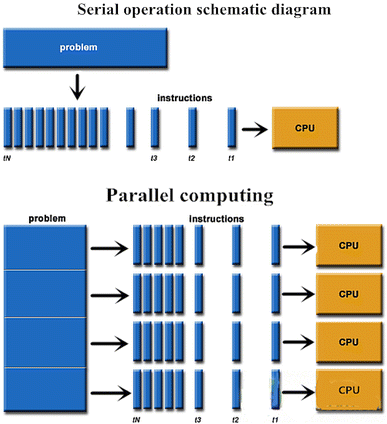
\includegraphics[width=\textwidth]{img/serial-parallel.png}
		{\hspace*{\fill}\tiny\textit{Forrás: ResearchGate}}
	\end{figure}
\end{columns}

\end{frame}